%!TEX root = ../thesis.tex
%*******************************************************************************
%******************************  5th  Chapter **********************************
%*******************************************************************************

\chapter{Experimental results}
\label{chap:xp}
% **************************** Define Graphics Path **************************
\ifpdf
    \graphicspath{{Chapter5/Figs/Raster/}{Chapter5/Figs/PDF/}{Chapter5/Figs/}}
\else
    \graphicspath{{Chapter5/Figs/Vector/}{Chapter5/Figs/}}
\fi


\section{Ill suited for domain adaptation} % (fold)
\label{sec:ill_suited_for_domain_adaptation}

\victor{Find out why this is does not work : \url{https://arxiv.org/pdf/1909.03081.pdf} ??}


\victor{La simulation est trop précise. cf resultat sur l'impossibilité de séparer les domaines créé}



\section{Forest robustness} % (fold)
\label{sec:forest_robustness}

\victor{Grad boost is robust because trees disagrees between themselves}


\section{Impossible to separate between domain} % (fold)
\label{sec:impossible_to_separate_between_domain}

\content{}


\section{Explore the theoretical limits}

\topic{On toy problems all methods achieve good or perfect inference}
\content{}

A complex link bounds the observables $\xx$ and the parameters (nuisance and interest).
It is impossible to completely reduce the dependency between $y|x$ et $\alpha$.
Hence impossible to reduce the systematic uncertainty to zero.

Here methods are compared to the best possible inference.


\subsection{Remarks} % (fold)
\label{sub:remarks}

Then the best way to reduce the systematic uncertainty is to improve calibration !


\subsection{1D toy} % (fold)
\label{sub:1d_toy}



\begin{figure}[htb]
  \centering
  \begin{subfigure}[t]{0.49\linewidth}
    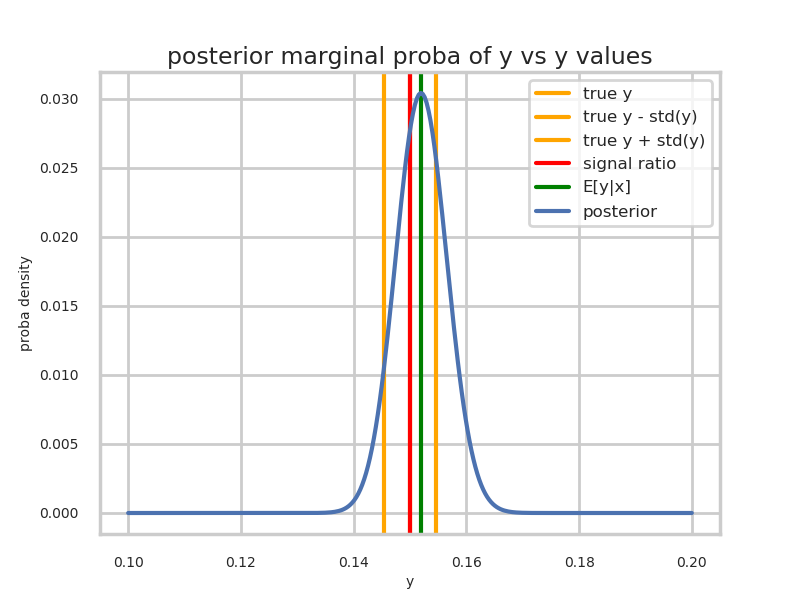
\includegraphics[width=\linewidth]{minitoy/marginal_y.png}
    \caption{$p(y|x)$}
    \label{fig:marginal_y}
  \end{subfigure}%
  \hfill
  \begin{subfigure}[t]{0.49\linewidth}
    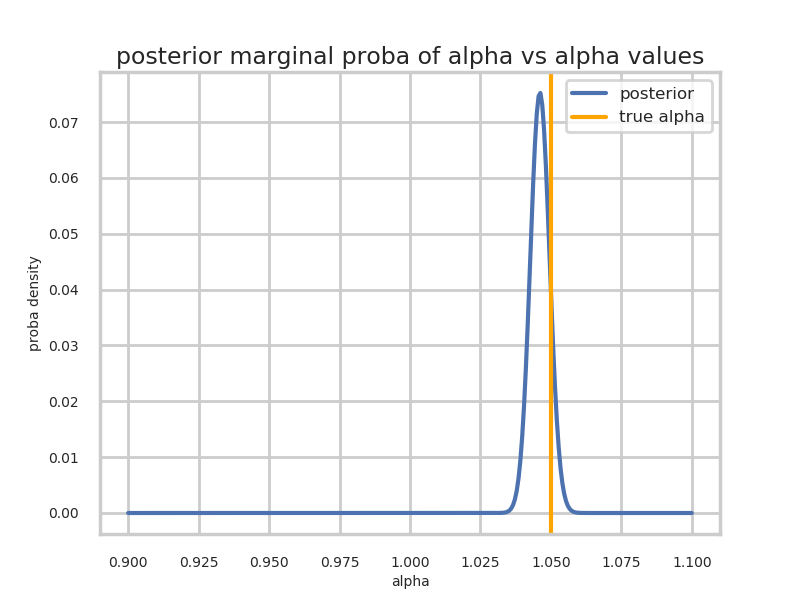
\includegraphics[width=\linewidth]{minitoy/marginal_alpha.png}
    \caption{$p(\alpha|x)$}
    \label{fig:marginal_alpha}
  \end{subfigure}
  \caption{Posterior probabilities for $y$ (left) and $\alpha$ (right)}
  \label{fig:marginals}
\end{figure}

\emph{Remarque :}
L'erreur statistique et l'erreur systématique diminuent ensemble avec l'augmentation du nombre de donnée.
Plus on a de donnée meilleur est l'inférence sur $\alpha$.
Donc c'est normal !

Du coup j'ai vraiment du mal avec le concepte de l'erreur systématique qui ne diminue que doucement avec l'augmentation des données.

Si l'effet est invisible sur les données alors on a pas de problème.
Si l'effet est visible alors on peut contraindre + les paramètres de nuisance puisqu'on peut le mesurer !


\subsection{3D toy} % (fold)
\label{sub:3d_toy}



\begin{figure}[htb]
  \centering
  \begin{subfigure}[t]{0.49\linewidth}
    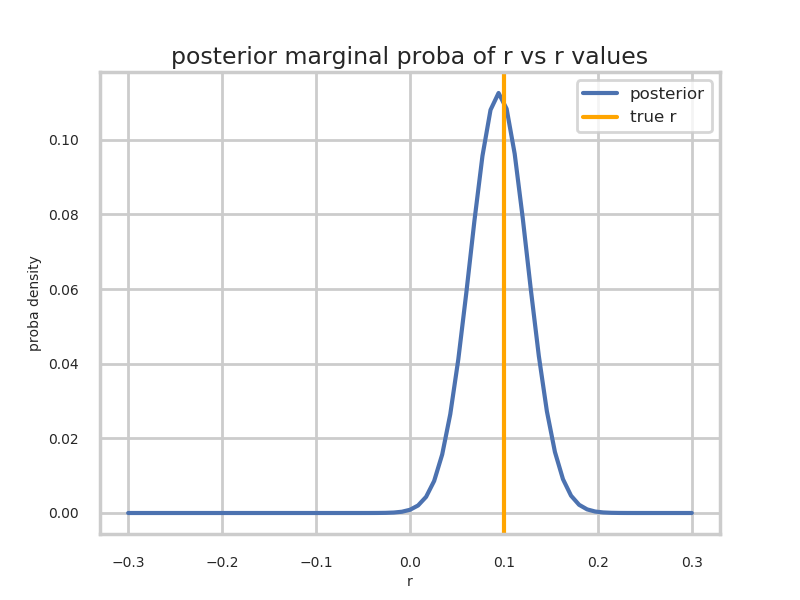
\includegraphics[width=\linewidth]{s3d2/marginal_r.png}
    \caption{$p(r|x)$}
    \label{fig:marginal_r}
  \end{subfigure}%
  \hfill
  \begin{subfigure}[t]{0.49\linewidth}
    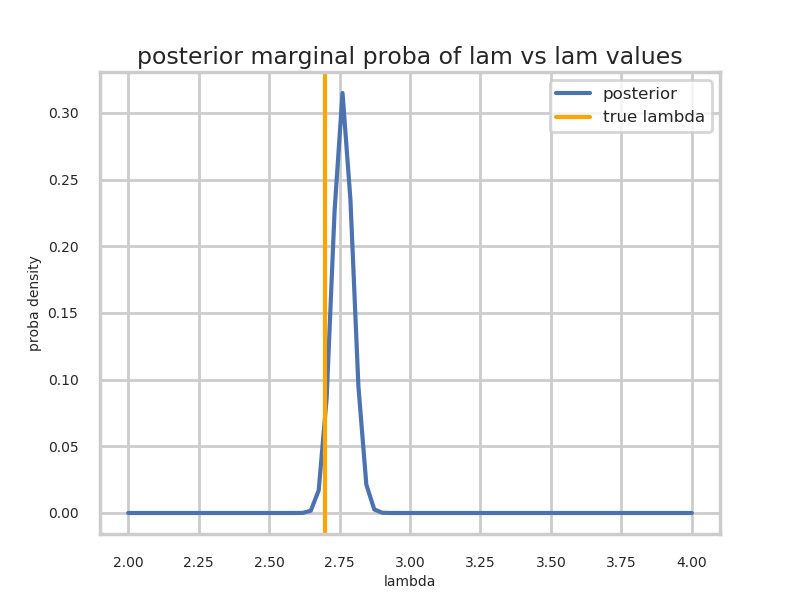
\includegraphics[width=\linewidth]{s3d2/marginal_lam.png}
    \caption{$p(\lambda|x)$}
    \label{fig:marginal_lambda}
  \end{subfigure}

  \begin{subfigure}[t]{0.49\linewidth}
    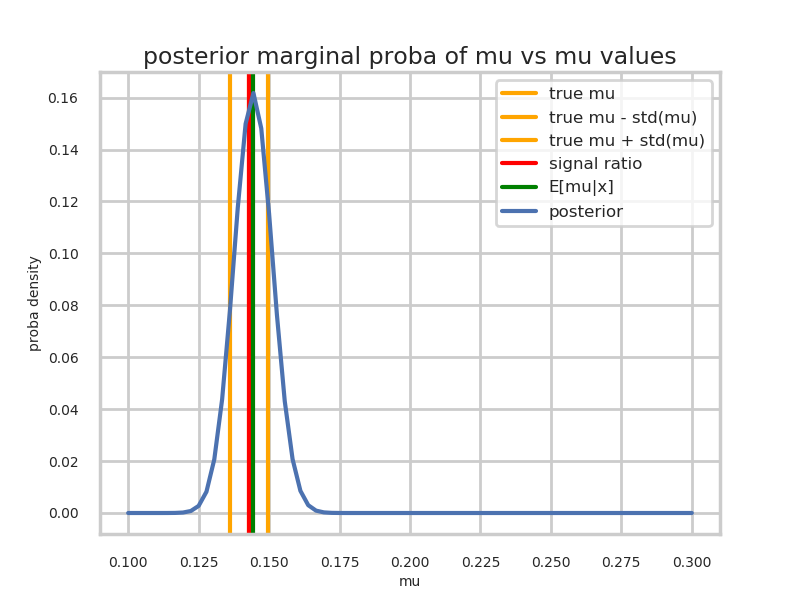
\includegraphics[width=\linewidth]{s3d2/marginal_mu.png}
    \caption{$p(\mu|x)$}
    \label{fig:marginal_mu}
  \end{subfigure}
  \caption{Posterior probabilities for $y$ (left) and $\alpha$ (right)}
  \label{fig:marginals}
\end{figure}






